\documentclass[11pt,a4paper,twoside,openright]{report}

\usepackage[top=25mm,bottom=25mm,right=25mm,left=30mm,head=12.5mm,foot=12.5mm]{geometry}
\usepackage[utf8]{inputenc}
\usepackage{tabularx}
\usepackage{multirow}
\usepackage{rotating} 
\usepackage{makecell}
\usepackage{array}
\usepackage{listings}
\let\openright=\cleardoublepage

\input{macros}

\def\NazevPrace{Arbitra}
\def\Trida{R8.A} 
\def\AutorPrace{Gabriel Hamrle}
\def\DatumOdevzdani{2026}

% Vedoucí práce: Jméno a příjmení s~tituly
\def\Vedouci{Emil Miler}

% Studijní program a obor
\def\StudijniProgram{studijní program}
\def\StudijniObor{studijní obor}

% Text čestného prohlášení
\def\Prohlaseni{Prohlašuji, že jsem svou práci vypracoval samostatně a použil jsem pouze prameny a literaturu
uvedené v~seznamu bibliografických záznamů. Nemám žádné námitky proti zpřístupňování této práce v~souladu se
zákonem č. 121/2000 Sb. o~právu autorském, o~právech souvisejících s~právem autorským a
o~změně některých zákonů (autorský zákon) ve znění pozdějších předpisů.}

% Text poděkování
\def\Podekovani{%
Poděkování.
}

% Abstrakt česky
\def\Abstrakt{%
Abstrakt.
}

% Abstrakt anglicky
\def\AbstraktEN{%
Abstract.
}

% 3 až 5 klíčových slov
\def\KlicovaSlova{extrahování dat, sázková kancelář, arbitrážní sázka, GET požadavek}
% 3 až 5 klíčových slov anglicky
\def\KlicovaSlovaEN{data extraction, betting shop, arbitrage bet, GET request}

\newcommand\yes{ANO}
\newcommand\no{NE}
\newcommand\nothing{--}
\newcommand{\head}[1]{\rotatebox{60}{\textbf{#1}}}

\begin{document}

\include{titlepage}

% Obsah
\setcounter{tocdepth}{2}
\tableofcontents
\chapter{Teoretická část}
\pagestyle{fancy}

V této části vysvětlím, jaká je motivace srovnávat kurzy napříč sázkovými kanceláři, co to je surebet a jak ho spočítat. Kdo docílil podobného výsledku a k tomu popíšu základní fungování webových stránek a jak z nich extrahovat data.

\section{Motivace}

Sázkové kanceláře vypisují kurzy na tisíce zápasů nezávisle na sobě, čímž vzniká nemalá šance, že některé z kurzů budou nesprávné – tj. jejich hodnota je vyšší než kurz vyplývající ze skutečné pravděpodobnosti. Díky tomu mohou dvě sázkové kanceláře vypsat na dvě opačné události kurzy natolik vysoké, že pokud člověk vsadí na oba výsledky určité množství peněz, vždy skončí v zisku. Tento fenomén se nazývá surebet nebo arbitrážní sázka. 

Další využití srovnávání kurzů se nabízí při plnění bonusů, kde je potřeba prosázet určité množství peněz, aby uživatel získal benefit, typicky ve formě freebetu (sázka zdarma), peněžního obnosu nebo freespinů. V těchto případech je žádoucí najít co nejméně ztrátovou sázku, což právě můj program umožňuje. 

Vědět o profitujících či méně ztrátových příležitostech je tedy klíčové, pokud chce člověk porazit sázkové kanceláře.

\subsection{Počítání arbitrážní sázky}

V této podsekci odvodím pár rovnic, které určí, zda-li mohu udělat surebet. Nechť mám události 1 a 2 s kurzy $k_1$ a $k_2$, přičemž jedna z nich se určitě stane. Pokud mám obnos $V$ a chci vsadit na obě události tak, abych vždy vyhrál (respektive prohrál) stejné množství peněz, musí na první vsadit $\frac{V}{k_1}$ a na druhou $ \frac{V}{k_2}$, přičemž abych profitovat, tak musí platit, že
\begin{equation}
	\begin{split}
	\frac{V}{k_1} + \frac{V}{k_2}  &< V \\
\Leftrightarrow \frac{1}{k_1} + \frac{1}{k_2} &< 1.
	\end{split}
\end{equation}

Zobecněním na $n$ kurzů dostaneme, že musí platit:

\begin{equation}
    \sum_{i=1}^n \frac{1}{k_i} < 1,
\end{equation}

kde $k_i$ je $i$-tý kurz na $i$-tý výsledek a alespoň jeden z výsledků 1 až $n$ vždy nastane. Zhodnocení původního vkladu $p$ lze spočítat následovně:

\begin{equation}
    p = \frac{1}{\sum_{i=1}^n \frac{1}{k_i}}.
\end{equation}

Vklad na $i$-tý kurz $V_i$ lze určit takto:

\begin{equation}
    V_i = \frac{V \cdot p}{k_i}.
\end{equation}


\section{Existující řešení}

Hledání surebetů není novinkou a v současnosti existuje několik webových stránek a projektů na platformě GitHub, které tuto službu poskytují. Ovšem nezahrnují všechny české sázkové kanceláře (tj. Tipsport, Chance, Fortuna, Betano, Allwyn, Synottip, Kingsbet, MerkurXtip) nebo jsou alespoň částečně placené. V následující tabulce uvádím šest takových webových stránek a sázkové kanceláře, ze kterých extrahují data. Také uvádím projekty na GitHubu, které se touto problematikou zabývají. Tyto projekty jsem vyhledával skrze vyhledávač Google, je tedy pravděpodobné, že jsem některé z nich mohl přehlédnout. Taktéž jsem netestoval jejich správnost. Zároveň se mi nepodařilo najít program, který by srovnával data z českých sázkových kanceláří a hledal arbitráže.

\begin{table}[h]
\centering
\small 
\noindent
\setlength{\tabcolsep}{3pt} 
\renewcommand{\arraystretch}{1.5} 

\begin{tabularx}{\textwidth}{|l||*{8}{>{\centering\arraybackslash}X|}c|}
    \hline
    \multicolumn{10}{|c|}{\rule{0pt}{15pt} \large \textbf{Vyhledávače surebetů – webové stránky}} \\ [1ex]
    \hline
    \rule{0pt}{45pt} \textbf{Web} & \head{Tipsport} & \head{Chance} & \head{Fortuna} & \head{Betano} & \head{Allwyn} & \head{Synottip} & \head{Kingsbet} & \head{MerkurXtip} & \head{Placený} \\
    \hline
    Oddspedia & \no & \no & \no & \yes & \no & \no & \no & \no & \no \\
    \hline
    Rebelbetting & \nothing & \nothing & \nothing & \nothing & \nothing & \nothing & \nothing & \nothing & \yes \\
    \hline
    BetBurger & \yes & \no & \yes & \no & \yes & \no & \no & \no & \yes \\
    \hline
    Arbmate & \nothing & \nothing & \nothing & \nothing & \nothing & \nothing & \nothing & \nothing & \yes \\
    \hline
    Oddsportal & \yes & \yes & \yes & \yes & \no & \no & \no & \no & \no \\
    \hline
    Surebet & \yes & \yes & \yes & \yes & \yes & \yes & \yes & \yes & \no* \\
    \hline
\end{tabularx}
\caption{Vyhledávače surebetů – webové stránky}
\begin{flushleft}
\footnotesize \nothing \ znamená, že daná stránka nemá transparentní údaje o tom, které sázkové kanceláře podporuje. \\
\footnotesize * Profit nad 1 \% se zobrazí pouze placeným členům.
\end{flushleft}
\end{table}

\begin{table}[h]
\begin{center}
\begin{tabularx}{\textwidth}{ | >{\raggedright\arraybackslash}m{6em}|| c | X | l | } 
\hline
\multicolumn{4}{|c|}{\rule{0pt}{15pt} \large \textbf{Vyhledávače surebetů – projekty na GitHubu}} \\ [1ex] 
\hline
    \textbf{Kancelář} & \textbf{Projekt?} & \textbf{Odkazy} & \textbf{Jazyk} \\
    \hline 
    \textbf{Tipsport} & \yes & \url{https://github.com/michalskop/tipsport.cz} & Python \\ 
    \hline
    \textbf{Chance} & \no & \nothing & \nothing \\ 
    \hline
    \textbf{Fortuna} & \yes & \url{https://github.com/michalskop/ifortuna.cz} & Python \\ 
    \hline
    \multirow{2}{5em}{\textbf{Betano}*} & \yes & \url{https://github.com/igormartins0301/projeto-scraping-betano} & Python \\ 
                                       & \yes & \url{https://github.com/hansalemaos/tutorial_raspagem_de_dados_betano/} & Python \\ 
    \hline
    \textbf{Allwyn} & \no & \nothing & \nothing \\ 
    \hline
    \textbf{Synottip} & \no & \nothing & \nothing \\ 
    \hline
    \textbf{Kingsbet} & \no & \nothing & \nothing \\ 
    \hline
    \textbf{MerkurXtip} & \no & \nothing & \nothing \\ 
  \hline
\end{tabularx}
\caption{Vyhledávače surebetů – projekty na GitHubu}
\begin{flushleft}
\footnotesize * Oba projekty jsou v portugalštině, a extrahují tedy data ze stránky betano.com, nikoliv betano.cz. To by ovšem nemělo vadit, neboť se jedná o tutéž platformu. 
\end{flushleft}
\end{center}
\end{table}

Jak lze vidět z tabulky webových stránek nabízejících zmíněnou službu, většina z nich uplatňuje restrikci na zobrazení surebetů pro neplatící uživatele. Můj program samozřejmě nemůže konkurovat profesionálním placeným službám jako surebet.com, představuje však open-source alternativu, ke které lze přidat moduly na extrahování dalších stránek, a zároveň zaručuje bezplatnou dostupnost. Největší nevýhodu svého programu oproti alternativám spatřuji v tom, že není schopen rozpoznat arbitráž pro jiné události než základní výsledek zápasů. Výhodou spuštění vlastního programu na lokálním počítači je naopak fakt, že si mohu sám určit frekvenci extrakce, čímž se snižuje šance, že zobrazená data budou zastaralá. \\

Pro svůj projekt jsem si vybral sázkové kanceláře Fortuna a Kingsbet, protože obě disponují API, které jsou snadno pochopitelné (viz následující část), a zároveň se na extrahování dat z Kingsbetu není open-source kód. Tento program jsem psal v programovacím jazyku C\#, protože jsem chtěl k extrakci zakomponovat rozhraní webové stránky, která se lépe programuje v ASP.NET frameworku, který existuje pouze pro C\#. Projekt by určitš´ě šel udělat i v pythnu, ale na větší projekty se podle mého uvážení nehodí. 

\section{Metody sběru dat z webové stránky}
Webové stránky vznikly za účelem vytvoření uživatelsky přívětivé a automatizované komunikace mezi uživatelem a organizací (např. firmou, univerzitou, školou atd.). V současné době se ustálil model, kdy si organizace pořídí nebo pronajme server a webovou adresu. Následně uživatel zadá danou adresu do prohlížeče a obdrží soubory od serveru, které se mu zobrazí jako webová stránka. Typicky obdrží HTML soubor se základní strukturou stránky, CSS soubory, které upravují vzhled HTML souboru, a JavaScriptové soubory, které definují interaktivní prvky stránky. Webové stránky dělíme na dva typy. \cite{gfg_webpage}\\

Pro jednoduchý přenos neměnných informací stačí takzvaná \textbf{statická webová stránka}, která je celá předpřipravená a po odeslání základních souborů již neinteraguje s databází. Tento způsob už v dnešní době není populární, ovšem pro jednoduché stránky s neměnnými daty může postačit. \\

Na složitější úkoly je potřeba využít tzv. \textbf{dynamickou webovou stránku}, která se odlišuje tím, že konzistentně komunikuje se serverem skrze požadavky (requesty), které aktualizují data na webové stránce, aniž by ji bylo nutné znovu načítat, respektive žádat o další web page request. Server k tomu využívá programovací jazyky typu PHP, ASP.NET či JSP, přičemž o komunikaci v prohlížeči se stará skript v JavaScriptu. \cite{gfg_dynamic} Všechny sázkové kanceláře mají dynamické webové stránky. \\

Většina dynamických webů disponuje API (Application Programming Interface), což je soubor funkcí umožňujících interakci se serverem. \cite{gfg_webapi} Nás bude zajímat situace, kdy klient obdrží data o kurzech, která se často (ale ne vždy) posílají ve formátu JSON (JavaScript Object Notation), a to nejčastěji skrze metody \textbf{GET} a \textbf{POST}. Jestliže identifikujeme správnou metodu, kterou náš prohlížeč využívá k zasílání kurzů ze serveru do našeho počítače, máme vyhráno, neboť takovou funkci můžeme spustit skrze jakýkoliv program a obdržíme tak přímo čistá data o kurzech.

\subsection{HTTP GET metoda}
Metoda HTTP GET žádá server o data bez dalších přidaných informací. Využívá se hlavně při zobrazení dat, která nejsou senzitivní a nepotřebují vstup (input) od uživatele. \cite{gfg_getpost} Často ji tedy využívají kanceláře k zobrazování aktuálních kurzů.

\subsection{HTTP POST metoda}
Na rozdíl od předchozího případu jsou součástí POST requestu data; jedná se tedy o požadavek se vstupem. \cite{gfg_getpost} Přestože není nezbytný, stránka \url{sport.synottip.cz} využívá metodu POST k přenosu kurzů. Součástí tohoto requestu je pak např. i token, který podle mých odhadů slouží k zamezení automatizovanému extrahování dat z webu skrze boty. 

\chapter{Implementace}

V této části uvedu, jak jsem nalezl vhodné GET mteody, přes které se posílají kurzy. 

\section{Nalézání vhodných GET metod}
Jak již bylo zmíněno v minulé části, většina webových stránek komunikuje se svým serverem skrze API. Tuto komunikaci lze vidět i v prohlížeči za pomocí Inspect tool. Následně popíšu, jak lze tuto komunikaci vidět v prohlížeči Firefox, přestože ostatní prohlížeče typu Google Chrome budou fungovat na velmi podobném počítači.

Po otevření dané stránky, kterou chceme prohledat klikneme kdekoliv na stránce pravým tlačítkem myši a zvolíme možnost Inspect. Následně v horní liště zvolíme Network, čímž uvidíme celou následující komunikaci mezi serverem a stránkou. Tedy předchozí requesty tam nevidíme. Otevření Network lišty lze také docílit za pomocí zkratky Ctrl + Shift + E. 

Poté musíme znovu načíst webovou stránku a počkáme, až se načtou všechny potřebné data, což jsou v našem případě kurzy. Následně zastavíme další záznam komunikace skrze tlačítko Pause s ikonoou II (viz. Obr.), aby se nám do toho nepletly např. requesty pro live sázky, které se každou chvílí aktualizují. Nyní vidíme všechnu komunikaci, přes kterou by se mohly kurzy posílat. 

Nejjednodušší případ se stává, když se zápasy posílají skrze Get metodu ve formátu JSON, který není jakkoliv kódovaný. Jak jsem zjistil, tak sázkové kanceláře Fortuna a Kingsbet využívají přesně tuhle metodu a tedy ukážu pouze co dělat v tomhle případě. 

Následně zaklikneme, že chceme vidět pouze XHR - XMLHttpRequest, čímž se nám zobrazí pouze requesty, který vrací nějakou strukturu dat. (VYSVĚTLIT LÍP) Dále tedy musíme prozkoumat každý z těchto requestů. Někdy mohou být pojmenovány tak, že jde poznat o co jde (např. GetEvents), ale nelze na to spoléhat. 

Když člověk klikne pravým tlačítkem myši na daný request a klikne na open in new tab, uvidí JSON formát, který z daného requestu dostanu a taky adresu, přes kterou request udělá. Pokud tímto způsobem rozkliknu několik requestů, které se podle jména zdají relevantní, uvidím několik souborů ve kterých musím nalézt systém jak fungují. Neexistuje jednoznačná metoda jak lze tento systém nazpátek zjistit, ovšem ukážu jak jsem ho zjistil u Fortuny a Kingsbetu, přičemž u ostatních kanceláří lze pravděpodobně dosáhnout stejného výsledku podobnou metodou, přestože to není zaručené.
 
 
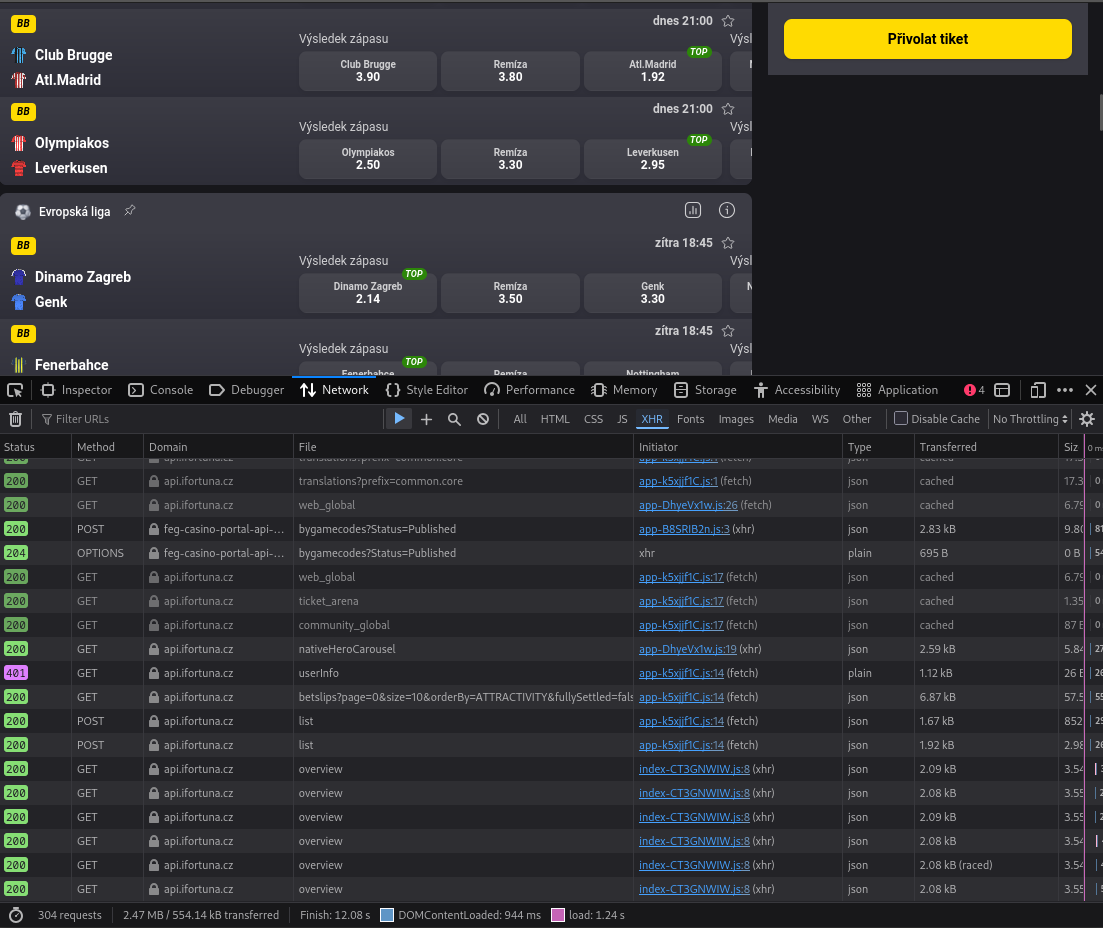
\includegraphics[width=\textwidth]{img/Fortuna.png} 

\section{Jak získat GET metodu v C\#}
Všechny soubory, které extrahují data z externích webů se nachází ve složce ./Background/MatchFinders. Soubor, který je spouští je OddsFinder.cs

V .NET prostředí lze využít objektu HttpClient, který umožňuje získat Get request na základě webové adresy. A to za pomocí GetAsync() metody. V rámci projektu jsem vytvořil funkci, která získává JsonNode z URL viz. Zde. 

Pro Kingsbet bylo potřeba obejít základní detekci proti robotům, což se vyřešilo přidáním request headrů pro všechny request. Viz kód 


\section{Struktura ukládání dat}
Všechny soubory, které tvoří strukturu ukládání zápasů, jsou ve složce ./Data Structure.

V rámci projektu jsem sbíral kurzy pouze na zápasy a to jenom na vítěze zápasu, případně na dvojtip (neprohra týmu). Obecná struktura všech událostí je mnohem složitější na uspořádání a tedy není implementovaná v mém projektu.

Match - Když se hledají zápasy, tak se ukládají podle této třídy, která obsahuje jméno zápasu, jméno týmu A, jméno týmu B, datum zápasu a tabulku kurzů, kde pro každý výsledek jsou uvedeny všechny různé kanceláře s kurzem a odkazem na zápas. Zároveň obsahuje funkci Merge, která spojí dva stejné zápasy do jednoho, aby objekt obsahoval informace o všech sázkových kanceláří.

ListOfMatches - list tříd Match s funkcí Merge(), která spojuje stejné zápasy, které najde v listu. Funkce SplitToEvents() (která se nachází i ve třídě Match) rozděluje zápasy na několik objektů třídy Event. 

Event - podobná struktura jako Match, ale může se stát pouze jeden výsledek z uvedených kurzů. Zároveň lze získat profit ze sázení na tyto události podle vzorců uvedených v motivaci. Taktéž lze tuto třídu serializovat a deserializovat do JSON objektu.

MatchOdds - jako Odds, ale s funkcí merge, která spojí dvě stejné 

Odd - kurz na konkrétní výsledek vypsaný konkrétní sázkovou kanceláří. Obsahuje kurz, sázkovou kanceláří, která kurz vypisuje, a odkaz na zápas. 

Odds - list tříd Odd, který uchovává všechny možné kurzy na jeden konkrétní výsledek zápasu. Obsahuje funkci Sort(), která seřadí kurzy od největšího.



\section{Rozpoznání stejných zápasů}
Ze zápasů jsem sbíral jména týmů a datum. Protože kanceláře mohou využívat jiný formát názvu týmu, rozhodl jsem se, že každý tým nazvu zkrácenou verzí, kterou vytváří funkce NormalizeString() v souboru /DataStructure/Match.cs.  Zároveň v tom stejném souboru funkce IsSame definuje, kdy jsou oba zápasy stejné. Aby byly, musí platit následující
\begin{enumerate}
\item Zkrácený název prvního týmu prvního zápasu je obsažen ve zkráceném názvu prvního týmu ve druhém zápasu, nebo naopak.\\
\item Zkrácený název druhého týmu prvního zápasu je obsažen ve zkráceném názvu druhého týmu ve druhém zápasu, nebo naopak.\\
\item Počet možností, jak zápas může skončit je stejný.\\
\item Čas, kdy se zápasy konají jsou stejné.\\
\end{enumerate}
Tento systém rozpoznání stejných zápasů je naprosto arbitrární a nezaručuje naprostou úspěšnost. Kvůli identitě času konání je pravděpodobnost na neúspěšnost relativně malá, ovšem pro budoucí vývoj je potřeba vymyslet více robustní metodu.

\section{Uživatelské rozhraní}
Jakožto uživatelské rozhraní jsem si vybral webovou stránku naprogramovanou v ASP.NET frameworku. Jedná se o populární a open source možnost jak tvořit webové stránky. Uživatel při otevření tohoto projektu tedy bude obeznámen s rozhraním pro něho známé, tj. rozhraní webových stránek, což je z mého pohledu přívětivější než rozhraní vlastní aplikace, případně výpisu z konzoly. Zároveň zakomponování tohoto projektu do webové stránky umožňuje budoucí uplatnění, pokud se někdy v budoucnu rozhodnu spouštět tento projekt na internet skrze server. 

Na hlavní stránce člověk uvidí všechny zápasy s primárními kurzy seřazené od nejvýdělečnějších kurzů, respektive od nejméně prodělečných. Daný kurz si člověk může rozkliknout, čímž se dostane na stránku daného zápasu dané sázkové kanceláře. Také si může rozkliknout zápas jako takový, čímž se dostane do Countru, který umožňuje spočítat, kolik na jaký kurz vsadit, aby byla sázka vždy stejně výnosná. 



\chapter{Technická dokumentace}
Projekt byl vytvořen v ASP.NET frameworku a je v něm zakomponovaný dockerfile, čímž je umožněno ho spustit v docker containeru. K spuštění je potřeba mít nainstalovaný git a docker. Dále stačí naklonovat repozitář do svého počítače a spustit ho v dockeru. Na linuxu toho lze docílit s těmito commandy: \\
\\
\begin{lstlisting}
	git clone https://github.com/Dxlaby/Arbitra
	
	cd Arbitra
	
	sudo docker compose up --build
\end{lstlisting}

Stránka nyní bude běžet přes port :8080 a tedy stačí navštívit stránku http://localhost:8080, (nikoliv https) případně http://[ip\_adresa]:8080 pro všechny uživatele dané sítě. 

Po spuštění chvíli trvá, než stránka načte kurzy a tedy se tam pár minut žádné nezobrazují. Následně lze vidět zápasy seřazené podle největšího profitu, respektive nejnižší ztráty. Po rozkliknutí daného zápasu lze vidět tzv. counter, který spočítá na jaký kurz máte vsadit kolik, aby jste vždycky vyhráli, respektive prohráli, stejné množství peněz. Zároveň ukáže celkový profit.

V konzoli se možná vypíšou errory ohledně nedostupného requestu. Ty pouze informují uživatele o faktu, že se kód snažil získat request, který neexistuje. Nejčastěji z důvodu, že se nějaká hodnota chybně označila jako např. ID turnamentu, zápasu apod. Nejedná se ovšem o chybu, která by naznačovala nefunkční systém. 



\chapter*{Závěr}
\pagestyle{empty}
\addcontentsline{toc}{chapter}{Závěr}

Závěr obsahuje shrnutí práce a vyjadřuje se k míře splnění jejího zadání. Dále by se zde mělo objevit sebehodnocení studenta a informace o tom, co nového se naučil a jak vnímal svou práci na projektu.

%%% Seznam použité literatury
% \nocite{einstein}\nocite{latexcompanion}\nocite{knuthwebsite}
\printbibliography[title={Seznam použité literatury},heading={bibintoc}]

%%% Seznam obrázků
\openright
\listoffigures
\addcontentsline{toc}{chapter}{Seznam obrázků}

%%% Seznam tabulek
\clearpage
\listoftables
\addcontentsline{toc}{chapter}{Seznam tabulek}

%%% Přílohy k práci, existují-li. Každá příloha musí být alespoň jednou
%%% odkazována z vlastního textu práce. Přílohy se číslují.

%\part*{Přílohy}
%\appendix

\end{document}
